\lecture{28}{12. Januar 2026}{2024 Exam}

\begin{problem}{1}
  Consider the situation shown in the figure, where a triangular steel plate (in yellow) is connected to a wall via a ball and socket joint at point $A$.
  The weight of the plate is \qty{500}{\N}, and the gravity force acts downward along the negative $y$ axis.
  To maintain equilibrium, the plate is also connected to two cables at points $B$ and $C$.
  The thickness of the plate can be assumed uniform and negligible in relation to the other geometrical dimensions.
  Therefore, points $A$, $B$ and $C$ can be considered to all lie on the $z$ axis,

  \begin{itemize}
    \item[Q1.1] Draw a free body diagram of the plate indicating all the forces acting on it.
    \item[Q1.2] Compute the unit vector along which the tension $\Vec{T}_1$ acts (directed from point $C$ along the cable)
    \item[Q1.3] Use moment equilibrium to find the magnitude of the tension $\Vec{T}_1$.
    \item[Q1.4] Use the remaining equilibrium equations to find all the other unknown forces acting on the plate.
  \end{itemize}

  Assume now that the cable connected at point $C$ can be considered a slender bar with circular cross-section, consisting of a steel core and an aluminum outer sell.
  The outer diameter of the cable is \qty{4}{\mm}, and the diameter of the steel core is \qty{2}{\mm}.

  \begin{itemize}
    \item[Q1.5] Calculate the elongation of the cable due to the tension $\Vec{T}_1$.
      The Young's modulus of steel and of aluminum can be assumed to be \qty{210}{\GPa}  and \qty{70}{\GPa} , respectively.
  \end{itemize}

  \begin{figure} [ht]
    \centering
    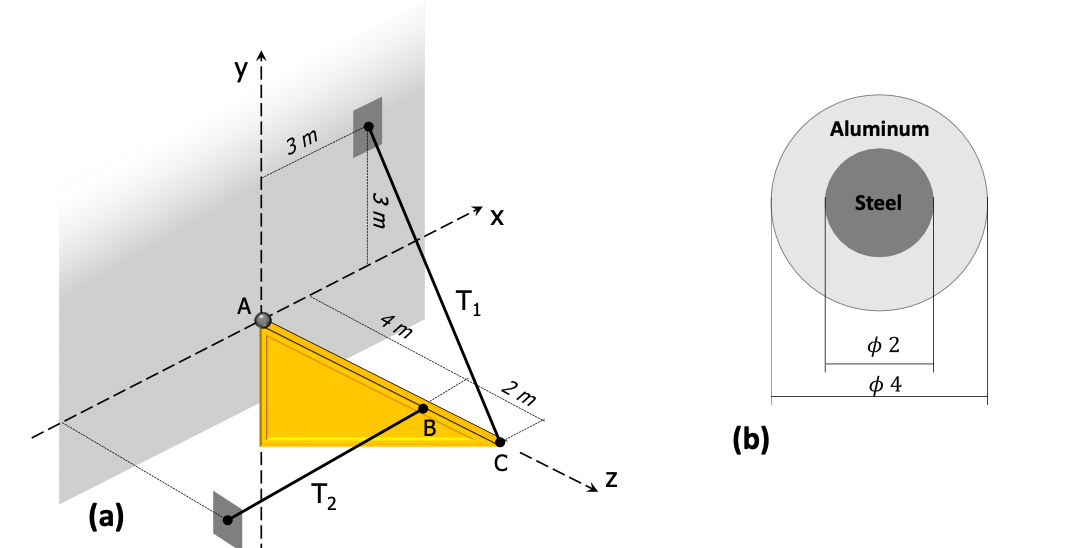
\includegraphics[width=0.8\linewidth]{./figures/e20241.png}
  \end{figure}
\end{problem}

\begin{derivation}
  \begin{itemize}
    \item[Q1.1] Two free-body diagrams (one in the $yz$ plane and one in the $xz$ plane) have been constructed and they can be seen on \Cref{fig:e20251fbd}.

      \begin{figure}[ht]
        \centering
        \incfig{e20251fbd}
        \caption{Free body diagram.}
        \label{fig:e20251fbd}
      \end{figure}
    \item[Q1.2] $\Vec{T}_1$ acts along the line from $C = (0; 0; \qty{6}{\m})$ to $D = (\qty{3}{\m}; \qty{3}{\m}; 0)$. This means that it acts along the vector:
      \begin{equation*}
        \Vec{CD} = D - C = (\qty{3}{\m}; \qty{3}{\m}; \qty{-6}{\m})
      .\end{equation*}
      A unit vector along this can now be found by dividing $\Vec{CD}$ by $\left| \Vec{CD} \right|$ as:
      \begin{align*}
        \hat{u}_{T_1} &= \hat{u}_{CD} \\
        &= \frac{(\qty{3}{\m}; \qty{3}{\m}; \qty{-6}{\m})}{\sqrt{\left( \qty{3}{\m}  \right)^2 + \left( \qty{3}{\m}  \right)^2 + \left( \qty{6}{\m}  \right)^2}} \\
        &= \left( \num{0,408}; \num{0,408}; \num{-0,816}   \right) \\
        &= \num{0,408} \Vec{i} + \num{0,408} \Vec{j} - \num{0,816} \Vec{k}
      .\end{align*}
    \item[Q1.3] We use a moment equilibrium about point $A$ in the $yz$ direction to obtain. Note that the center of gravity of the steel plate will lie at $z = \qty{2}{\m} $ as it is a triangle.
      Hence:
      \begin{align*}
        \sum \left( M_A \right)_{yz} &= 0 \\
        T_{1y} \cdot \qty{6}{\m}  - W \cdot \qty{2}{\m} &= 0 \\
        T_{1y} &= \frac{\qty{500}{\N}  \cdot \qty{2}{\m} }{\qty{6}{\m} } \\
        &= \qty{166,67}{\N}
      .\end{align*}
      Using the unit vector we can then find the magnitude of $T_1$ as
      \begin{equation*}
        \Vec{T}_1 = \frac{T_{1y}}{(\hat{u}_{T_{1}})_y} = \frac{\qty{166.67}{\N}}{\num{0.408} } = \qty{408,5}{\N}
      .\end{equation*}
    \item[Q1.4]  Using a global force equilibrium in the $y$ direction we obtain the reaction $A_y$ as:
      \begin{align*}
        \sum F_y &= 0 \\
        A_y - W + F_{1y} &= 0 \\
        A_y &= -\qty{166,67}{\N} + \qty{500}{\N}  \\
        A_y &=  \qty{333,33}{\N} 
      .\end{align*}
      A force equilibrium in the $z$ direction yields:
      \begin{align*}
        \sum F_z &= 0 \\
        A_z - F_{1z} &= 0 \\
        A_z &= F_{1z} \\
        A_z &= \qty{408,5}{\N} \cdot \num{-0,816}  \\
        A_z &= \qty{-333,336}{\N} 
      .\end{align*}
      And in the $x$ direction we get:
      \begin{align*}
        \sum F_x &= 0 \\
        A_x - T_2 + T_{1x} &= 0 \\
        A_x - T_2 &= - T_{1x} \\
        A_x - T_2 &= - \qty{408.5}{\N} \cdot \num{0,408} \\
        A_x - T_2 &= - \qty{166,668}{\N} 
      .\end{align*}
      And now we use a moment equilibrium about $A$ in the $xz$ direction to get:
      \begin{align*}
        \sum \left( M_A \right)_{xz} &= 0 \\
        - T_2 \cdot \qty{4}{\m} + T_{1x} \cdot \qty{6}{\m} &= 0 \\
        T_2 &= \frac{T_{1x} \cdot \qty{6}{\m} }{\qty{4}{\m} } \\
        T_2 &= \frac{\qty{166,67}{\N} \cdot \qty{6}{\m} }{\qty{4}{\m} } \\
        T_2 &= \qty{250}{\N} 
      .\end{align*}
      Which means that:
      \begin{equation*}
        A_x = - \qty{166,668}{\N} + \qty{250}{\N} = \qty{83,332}{\N} 
      .\end{equation*}
      I.e.
      \begin{align*}
        A_x &= \qty{83,33}{\N}  \\
        A_y &= \qty{333,33}{\N}  \\
        A_z &= \qty{-333,33}{\N}  \\
        T_2 &= \qty{250}{\N}
      .\end{align*}
    \item[Q1.5] For there to be no sliding between the aluminum and steel layers we require $\epsilon_{st} = \epsilon_{al} = \epsilon$.
      Hence,
      \begin{equation*}
        \sigma_{\mathrm{st}} = E_{\mathrm{st}} \epsilon \qquad \sigma_{\mathrm{al}} = E_{\mathrm{al}} \epsilon
      .\end{equation*}
      The force is then
      \begin{equation*}
        T_1 = \sigma_{\mathrm{st}} \cdot A_{\mathrm{st}} + \sigma_{\mathrm{al}} \cdot A_{\mathrm{al}} = \epsilon \left( E_{\mathrm{st}} A_{\mathrm{st}} + E_{\mathrm{al}} A_{\mathrm{al}} \right)
      .\end{equation*}
      So,
      \begin{align*}
        \epsilon &= \frac{T_1}{E_{\mathrm{st}} \cdot \pi \cdot \frac{\left( \qty{2}{mm}  \right)^2}{4} + E_{\mathrm{al}} \cdot \pi \cdot \frac{\left( \qty{4}{\mm}  \right)^2 - \left( \qty{2}{\mm}  \right)^2}{4}} \\
                 &= \frac{\qty{408.5}{\N} }{\qty{210}{\GPa} \cdot \pi \cdot \frac{\left( \qty{2}{\mm}  \right)^2}{4} + \qty{70}{\GPa} \cdot \pi \frac{\left( \qty{4}{\mm}  \right)^2 - \left( \qty{2}{\mm}  \right)^2}{4}} = \num{3,096e-4}
      .\end{align*}
      So the elongation is:
      \begin{equation*}
        \delta = \left| CD  \right| \epsilon = \sqrt{\qty{9}{\m^2} + \qty{9}{\m^2} + \qty{36}{\m^2}} \cdot \num{3,096e-4} = \qty{2,28}{\mm}  
      .\end{equation*}
  \end{itemize}
\end{derivation}

\finalresult{
\begin{aligned}
  &\mathrm{Q1.1} & &\text{See \Cref{fig:e20251fbd}} \\
  &\mathrm{Q1.2} & \hat{u}_{T_1} &= \num{0,408} \Vec{i} + \num{0,408} \Vec{j} - \num{0,816} \Vec{k} \\
  &\mathrm{Q1.3} & T_1 &= \qty{408,5}{\N}  \\
  &\mathrm{Q1.4} & A_x &= \qty{83,33}{\N}  A_y = \qty{333,33}{\N} \\
  && A_z &= \qty{-333,33}{\N} T_2 = \qty{250}{\N}  \\
  &\mathrm{Q1.5} & \delta &= \qty{2,28}{\mm}
.\end{aligned}
}

\begin{problemwithimage}{e20242}{2}
  Consider a steel T-section overhand beam loaded as shown in Fig. 2.

  Let $L = \qty{4}{\m}$, $l = \qty{1}{\m}$, $w_0 = \qty{4}{\kN\per\m}$, $E= \qty{200}{\GPa} $, $t = \qty{10}{\mm}$, $f = \qty{15}{\mm}$, $b = h = \qty{300}{\mm}$.

  \begin{itemize}
    \item[Q2.1] List all reactions and kinematic constraints, establish whether the structure is statically determinate or indeterminate, and find its degree of indeterminacy.
    \item[Q2.2] Find the reaction forces and derive expressions for the shear force and bending moment along the beam.
    \item[Q2.3] On the cross section located at $x = L / 2$, draw the Mohr circle at point C and find the principal stresses and directions. (You may want to start by finding the state of stress at point $C$).
  \end{itemize}

  We replace the support at $A$ by a fixed support -- See Fig. 3.

  \begin{itemize}
    \item[Q2.4] Find the degree of indeterminacy of the structure and compute the reactions at $A$ and $B$.
  \end{itemize}
\end{problemwithimage}

\begin{derivation}
  \begin{itemize}
    \item[Q2.1] As $A$ is a pin it has reactions $A_x, A_y$ and the roller $B$ contributes a reaction of $B_y$. We have the boundary condition at $A$ that there can be no translation here, hence $v(0 ) = 0$ and the same is true at $B$ $v(L) = 0$. As we have three unknowns ($A_x$, $A_y$ and $B_y$) and three equilibrium equations ($\sum F_x = 0$, $\sum F_y = 0$, $\sum M = 0$) the structure is statically determinate.
    \item[Q2.2] We start by replacing the distributed load by a corresponding point loading.
      As the distributed load is triangular the point load will have a magnitude of
      \begin{equation*}
        W_0 = w_0 L = \frac{1}{2} \cdot  \qty{-4}{\kN\per\m} \cdot \qty{1}{\m} = \qty{-2}{\kN} 
      .\end{equation*}
      This will act directly downwards at $x = L + 2l / 3 = \qty{4}{\m} + \qty{0,666}{\m} = \qty{4,666}{\m}$.
      A force equilibrium in the $y$ direction then gives:
      \begin{align*}
        \sum F_y &= 0 \\
        A_y + B_y - W_0 &= 0 \\
        A_y + B_y &= W_0 \\
        A_y + B_y &= \qty{2}{\kN}
      .\end{align*}
      And a moment equilibrium about $A$ yields:
      \begin{align*}
        \sum M_A &= 0 \\
        B_y \cdot L - W_0 \cdot \qty{4,666}{\m} &= 0 \\
        B_y &= \frac{W_0 \cdot \qty{4,666}{\m} }{L} \\
        B_y &= \frac{\qty{2}{\kN} \cdot \qty{4,666}{\m} }{\qty{4}{\m} } \\  
        B_y &= \qty{ 2,333}{\kN} 
      .\end{align*}
      Which means
      \begin{equation*}
        A_y = \qty{2}{\kN} - \qty{2,333}{\kN} = -\qty{0,333}{\kN} 
      .\end{equation*}
      Hence, our shear diagram is defined by:
      \begin{equation*}
        V(x) = \begin{cases}
          A_y, & 0 \leq x \leq L\\
        A_y + B_y - \int_{L}^{x} w(s) \, \mathrm{d}s,  & L\leq x \leq L + l
        .\end{cases}
      .\end{equation*}
      We know that $A_y + B_y = W = \qty{2}{\kN}$ and $w(s) = \frac{w_0}{l}(s-L)$
      So
      \begin{align*}
        \int_{L}^{x} w(s) \, \mathrm{d}s &= \int_{L}^{x} \frac{w_0}{l}(s-L) \, \mathrm{d}s \\
        &= \frac{w_0}{2l}(x-L)^2 \\
        \frac{w_0 l}{2} - \frac{w_0}{2l} \left( x- L \right)^2 &= \frac{\qty{4}{\kN\per\m} \cdot \qty{1}{\m} }{2} - \frac{\qty{4}{\kN\per\m} }{2 \cdot \qty{1}{\m}} \left( x - \qty{4}{\m}  \right)^2  \\
        V(x) &= \begin{cases}
          - \qty{0,333}{\kN}  &  0 \leq x \leq L \\
        \qty{2}{\kN} - \qty{2}{\kN\per\m^2}  \left( x - \qty{4}{\m}  \right)^2 & L \leq x\leq L + l
        .\end{cases}
      .\end{align*}
      We use $M'(x) = V(x)$ and $M(0) = 0$ to get
      \begin{equation*}
        M(x) = \begin{cases}
          A_yx, & 0 \leq x \leq L\\
        A_y L + \int_{L}^{x} V(s) \, \mathrm{d}s & L\leq x \leq L+ l
        .\end{cases}
      .\end{equation*}
      Where we get:
      \begin{align*}
        \int_{L}^{x} V(s) \, \mathrm{d}s &= \int_{4}^{x} 2 - 2 \left( s - 4 \right)^2 \, \mathrm{d}s \\
          &= -\frac{2 x^3}{3}+8 x^2-30 x+\frac{104}{3}
      .\end{align*}
      Which means:
      \begin{equation*}
        \begin{cases}
          \num{0,333} x & 0 \leq x \leq L\\
        - \num{0,333} x - \frac{2x^3}{3} + 8 x^2 - 30 x + \frac{104}{3} & 
        .\end{cases}
      .\end{equation*}
      These are plotted on \Cref{fig:e20242sm}
      \begin{figure} [ht]
        \centering
        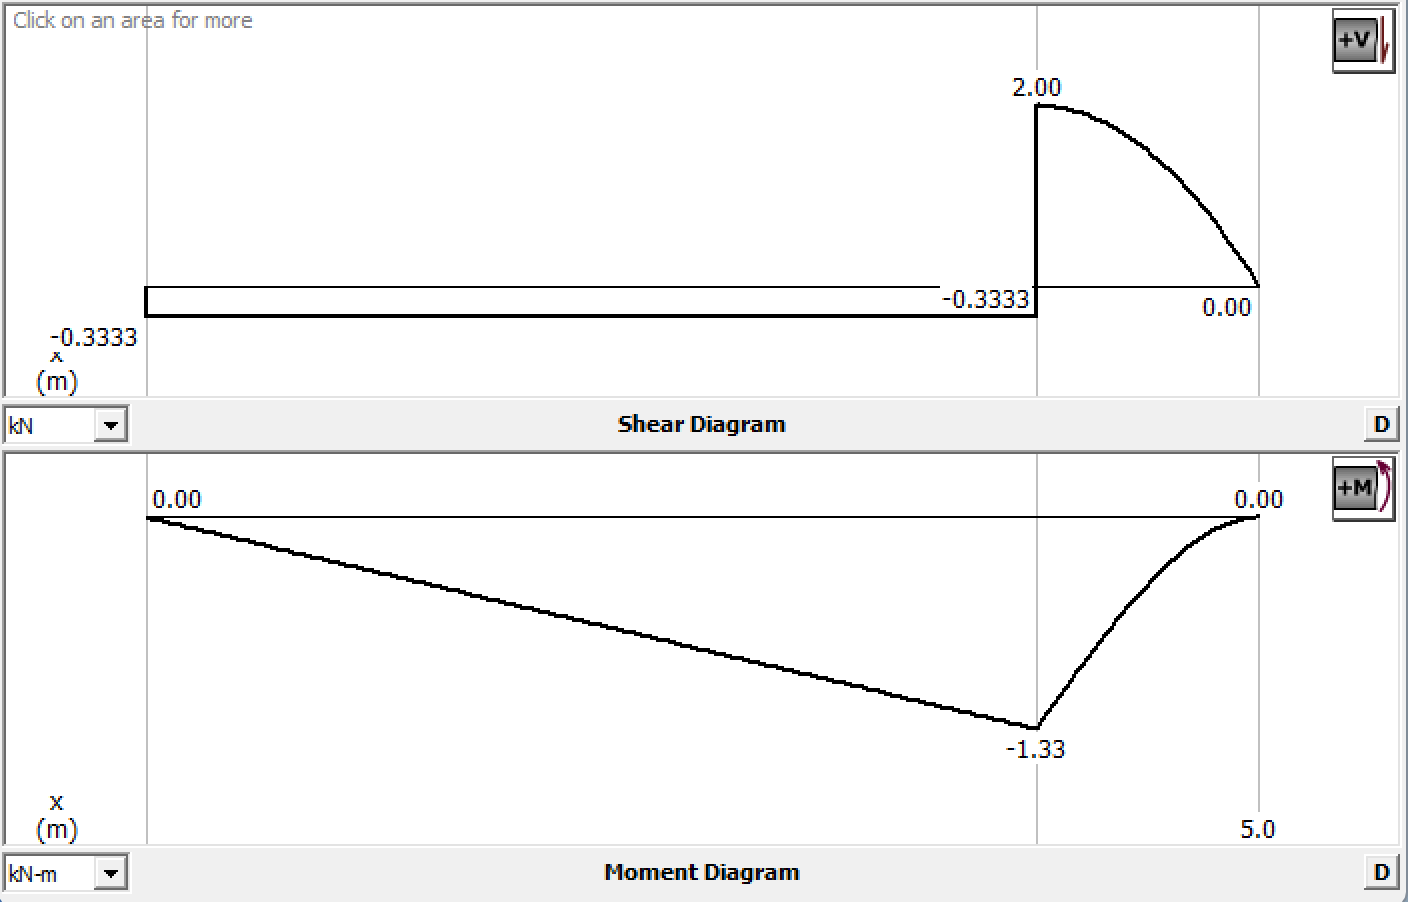
\includegraphics[width=0.8\linewidth]{./figures/e2025r1sm.png}
        \caption{Shear and Moment diagram.}
        \label{fig:e20242sm}
      \end{figure}
    \item[Q2.3]
    \item[Q2.4]Tissemand
  \end{itemize}
\end{derivation}
